\newpage

\subsection{Décodeur 7seg}

\begin{figure}[ht]
    \centering
    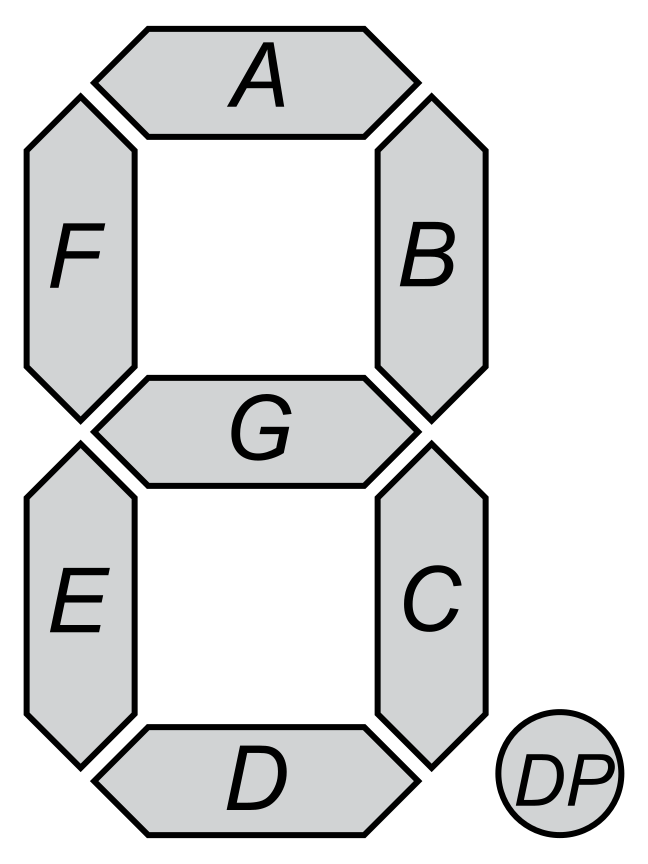
\includegraphics[scale = 0.1]{img/SevenSegDisplay.png}
    \caption{Segments d'un afficheur}
\end{figure}

Un afficheur sept segments est utilisé pour afficher des informations vers un utilisateur en allumant une partie des segments. Par exemple, pour afficher le chiffre \textit{2}, on allume les segments \textit{A, B, D, E, G}.

\medskip

- On veut afficher sur l'afficheur les chiffres allant de $0_h$ à $F_h$. Combien de bits il faut en entrée et en sortie pour pouvoir représenter ces chiffres.

\medskip

- Décrire la table de vérité de l'afficheur sept segments pour les chiffres allant de \textbf{$0_d$ à $F_d$.}

\medskip

- Décrire l'entité \textbf{seven\_segment} et l'architecture \textbf{rtl} de votre table de vérité en VHDL. 

\textbf{Note: Décrire les segments A, B, C, D, E, F comme un vecteur.}

\medskip

- Simuler et vérifier le bon comportement de votre table de vérité.

\medskip

- Connecter les entrées de votre décodeur sept segments aux switchs (SW$x$) et les sorties aux afficheurs sept segments (HEX$x$) de la carte DE2. Tester et vérifier le bon fonctionnement.

\medskip

- Expliquer pourquoi les bons segments sont éteints? Instancier le composant \textit{seven\_segment} à un module top level ou faire les modifications nécessaires au composant \textit{seven\_segment} pour que les bons segments s'allument.
